% filename GenericSettings.Rnw 



% filename Calculus001.Rnw 

% simplify, substitute factorise etc. 
% uniroot 
 
%\setcounter{chapter}{} 
\chapter{LURN\ldots{} To Use R for Basic Calculus Tasks} 
\label{Calculus} 
 
% filename Calculus002.Rnw 


% filename Calculus003.Rnw 

 
This chapter explains how various tasks in introductory calculus can be undertaken using \R{}. 
 
 
\section{Creating mathematical expressions} 
 
Before we embark on doing those fun things we want to do, we need to learn how to store a mathematical expression as an object in \R{}. There are many keywords that appear in these expressions which are translated to symbols when seen printed in a graph window but remain in ordinary text in \R{} commands. Such symbols include Greek letters, hats and bars, all of which have a meaning. 
 
\section{Plotting functions} 
 
This can be a lot of fun if you set things up right to start with. We create a \Rclass{function} to represent the mathematical expression using the \Rcmd{function} command, then plot it using either the \Rcmd{plot.function} or \Rcmd{curve} commands. 
% filename Calculus004.Rnw 

\begin{Schunk}
\begin{Sinput}
> MySine <- function(x){ sin(x)} 
> curve(MySine, -4*pi, 2*pi, n = 2001) 
\end{Sinput}

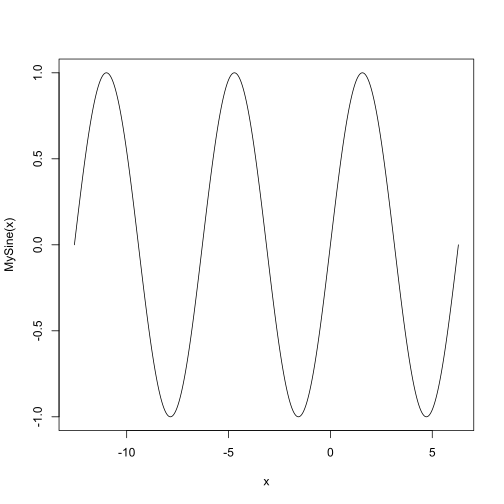
\includegraphics[width=0.7\textwidth]{figures/CalculusSineCurve-1} \end{Schunk}
% filename Calculus005.Rnw 

\SVGLink{CalculusSineCurve-1} 
 
You can use any valid mathematical expression in the \Rclass{function} you create. You might find it useful to test your idea= values for your inputs that are easy to work with, such as zero and one. You could then use integers, including negative integers, but  it could be easier to test your functions using values that lead to identifiable results such as multiples of $\pi$ when working with trignometric functions. For example: 
% filename Calculus006.Rnw 

<<EvalMySine>> 
MySine(c((0:4)*pi/2)) 
@ 
% filename Calculus007.Rnw 

 
%\section{} 
%\section{} 
 
 
\section{Differentiation} 
 
The internal code used for differentiation in \R{} is not as comprehensive as other mathematical software. 
It can handle arithmetic operators $+$, $-$, $*$, $/$ and \^, and the single-variable functions \Rcmd{exp}, \Rcmd{log} (natural logarithm), \Rcmd{sin}, \Rcmd{cos}, \Rcmd{tan}, \Rcmd{sinh}, \Rcmd{cosh}, \Rcmd{sqrt}, \Rcmd{pnorm}, 
\Rcmd{dnorm}, \Rcmd{asin} (inverse sine), \Rcmd{acos} (inverse cosine), \Rcmd{atan} (inverse tangent), and various \Rcmd{gamma} functions. The functions \Rcmd{pnorm} and \Rcmd{dnorm} are restricted to the standard normal distribution. 
 
The easiest way to find the derivative of an expression is to store the mathematical function using the \Rcmd{expression} command, and then use the \Rcmd{D} or \Rcmd{deriv} commands. 
% filename Calculus008.Rnw 

\begin{Schunk}
\begin{Sinput}
> y=expression(exp(2*x)) 
> D(y,"x") 
\end{Sinput}
\begin{Soutput}
exp(2 * x) * 2
\end{Soutput}
\end{Schunk}
% filename Calculus009.Rnw 

The second argument to the \Rcmd{D} function needs quote marks around it. 
 
% filename CleanUp.Rnw 



